\documentclass[jou]{apa6}

\usepackage[american]{babel}

\usepackage{csquotes}
\usepackage[style=apa,sortcites=true,sorting=nyt,backend=biber]{biblatex}
\DeclareLanguageMapping{american}{american-apa}
\addbibresource{bibliography.bib}


%%%%%%%%%%%%%%%%%%%%%%%%%%%%%%%%%%%%%%%%
%% Discrete Structures
%% The start of RBS stuff
%%%%%%%%%%%%%%%%%%%%%%%%%%%%%%%%%%%%%%%%

% Working internal and external links in PDF
\usepackage{hyperref}
% Extra math symbols in LaTeX
\usepackage{amsmath}
\usepackage{gensymb}
\usepackage{amssymb}
% Enumerations with (a), (b), etc.
\usepackage{enumerate}
\usepackage{xcolor}

\let\OLDitemize\itemize
\renewcommand\itemize{\OLDitemize\addtolength{\itemsep}{-6pt}}

\usepackage{etoolbox}
\makeatletter
\preto{\@verbatim}{\topsep=3pt \partopsep=3pt }
\makeatother

% These sizes redefine APA for A4 paper size
\oddsidemargin 0.0in
\evensidemargin 0.0in
\textwidth 6.27in
\headheight 1.0in
\topmargin -24pt
\headheight 12pt
\headsep 12pt
\textheight 9.19in



\title{Sample Quiz 4}
\author{Discrete Structures, Spring 2020}
\affiliation{RBS}

\leftheader{Discrete Quiz 7}

\abstract{%
}

%\keywords{}

\setlength\parindent{0pt}

\begin{document}

\thispagestyle{empty}

\twocolumn
{\Large Discrete Quiz 7}

% P1: 4+4 

\vspace{10pt}
{\bf Question 1 (Placing 8 rooks).} Somebody has an $8 \times 8$ chessboard and 
$8$ rooks ($4$ of them black, $4$ of them white). 
In how many ways one can place these $8$ rooks on the chessboard so that 
no rook shares the same horizontal or vertical with any other rook. 
Assume that the rooks of the same color are not distinguishable (but the chessboard itself cannot be rotated 
or flipped - i.e.\ we count symmetric positions multiple times).
\begin{center}
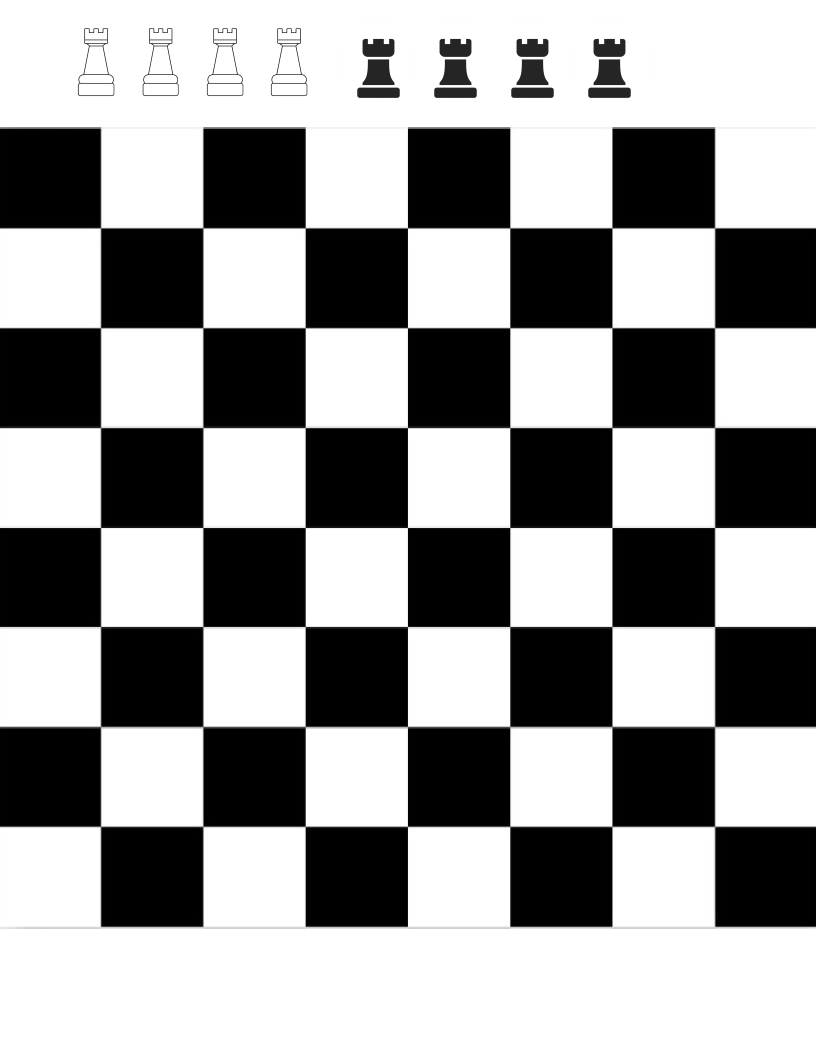
\includegraphics[width=2in]{quiz7/chessboard.png}
\end{center}

Write your answer as an integer number. 



\vspace{6pt}
{\bf Question 2 (Finding a higher order derivative).}\\
There is a formula to compute the 1st derivative of a product: 
$$(uv)' = u'v + v'u.$$
Assume that you need to compute the 4th derivative of a product of two functions $u\cdot v$. 
Enter the formula to compute $(uv)''''$. 

Your answer can use letters $u$, $v$, 
apostrophes (denoting the derivatives of the 1st, 2nd, 3rd and 4th degree), 
asterisk {\tt *} denoting multiplication and integer numbers. 


\vspace{6pt}
{\bf Question 3 (Multinomial formula).}\\
As a generalization to the Newton's binomial theorem (the expression for $(a+b)^n$), there
is also a more general {\em multinomial theorem}: 
$$(x_1 + x_2  + \cdots + x_m)^n
 = \sum\limits_{k_1+k_2+\cdots+k_m=n} {n \choose k_1, k_2, \ldots, k_m}
  \prod_{t=1}^m x_t^{k_t}\,,$$
where the {\em multinomial coefficients} are computed like this:
$${n \choose k_1, k_2, \ldots, k_m}
 = \frac{n!}{k_1!\, k_2! \cdots k_m!}$$

Assume that you use the multinomial formula to open parentheses in the following expression $(a+b+c)^9$.\\
{\bf (A)} How many {\em terms} are added in this expression?  (A term is a product 
of some number with the powers: $k\cdot a^x b^y c^z$, where $k$ is a positive number, but 
$x,y,z$ are nonnegative integers.)\\
{\bf (B)} What is the coefficient for the term $a^3b^3c^3$ in this expansion?

Write two numbers separated by a comma.




\vspace{6pt}
{\bf Question 4 (Permutations of ANNA).} Create a list of all permutations
of the letters in the word {\tt ANNA}. Assume that both copies of "A" and "N" are indistinguishable. 

Write an alphabetically sorted list separated by commas.


\vspace{6pt}
{\bf Question 5 (Pennies in jars).} 
Somebody has 5 pennies and 4 jars. All pennies are distinguishable and each penny should go into some jar. 
All the jars are placed in the vertices of a square $ABCD$; jar locations that differ only by rotations of that
square are considered indistinguishable. (For example, if all the pennies from the vertex $A$ would go to $B$; 
all pennies from $B$ would go to $C$, from $C$ to $D$, and from $D$ to $A$, then it would be the same way to distribute pennies.)

Find the number of ways how the pennies can be distributed among these jars. Write your answer as an integer.



\vspace{6pt}
{\bf Question 6 (Odd binomial coefficients).} Assume the following Kummer's theorem (\url{https://bit.ly/38Bak99}):\\
The binomial coefficient ${n \choose k} = C_n^k = \frac{n!}{k!(n-k)!}$ is odd iff
adding the binary notations of $k$ and $n-k$ there are no carries.\\ 
For example, the binomial coefficients ${10 \choose k}$ where $k=0,\ldots,10$ are the following:
$$\textcolor{red}{1},10,\textcolor{red}{45},120,210,252,210,120,\textcolor{red}{45},10,\textcolor{red}{1}.$$
The only odd numbers are ${10 \choose 0}$, ${10 \choose 2}$, ${10 \choose 8}$, ${10 \choose 10}$, 
since $0_{2} + 1010_{2}$ and also $10_{2} + 1000_{2}$ can be added without any carries (i.e.\
adding these we won't run into situation where we need to add $1+1$ or $1+1+1$ anywhere: Every situation 
where some digit is ``carried over'' from a smaller position of the binary number to a larger one is called a ``carry''.)

Find the number of odd numbers ${2020 \choose k}$, where $k = 0,1,\ldots,2020$. 
Express your answer as an integer number in decimal notation.


\vspace{6pt}
{\bf Question 7 (Sorted permutations).} As we know there are $5! = 120$ ways how to write the 5-letter word
{\tt ABCDE} (using every letter exactly once). Find the word that is written in the 100th position (assuming that
all the 120 permutations are sorted alphabetically).

Write your answer as 5-letter word.


\end{document}

